We compared performance of several algorithms against performance of algorithms in \cite{vamplew_potential-based_2021}. These were compared using the same environments and benchmarks as in \cite{vamplew_potential-based_2021}. Specifically, the environments were the UnbreakableBottles environment, the BreakableBottles environment, the Sokoban Environment, and the Doors environment.
\subsection{Testing environment}

We used a modified version of the testing environment from \cite{vamplew_potential-based_2021}, obtained with permission from the authors. There were several key changes for our implementation. Technical changes are not described here. Changes affecting modeling results themselves are described below.



\subsection{Aggregation functions}



All of the multi-objective utility functions we compared first follow the following basic steps:
\begin{enumerate}

    \item Apply an objective specific scaling factor $c$ which is multiplied with the value of the reward. The scaling factor is always same per objective, but different objectives likely have different scaling factors.
    \item Transform the scaled output using a non-linear transform. %For SFMLA, SFLLA, ELA, LELA, and SEBA, the transform is applied independently for each objective. % this is for ALL of the studied functions, right?
    \item Combine the transformed output using MEU.
\end{enumerate}

Each transform function is applied in the context of an aggregation function of the form

\begin{align}
\label{eq:meu}
U=\sum_{i}^n{f_i(x_i)}
\end{align}

\noindent where ${f_i(x_i)}$ describes a specific transform function for the $i$th objective. The SEBA transform function envisages differing functions for two categories of objectives. All other transform functions do not distinguish categories of objectives, and apply the same function over all objectives.


 New non-linear transforms compared were:

\begin{itemize}
    %\item Split-function multiplicative loss aversion (SFMLA)
    \item Split-function exp-log loss aversion (SFLLA)
    \item Exponential loss aversion (ELA)
    \item Linear-exponential loss aversion (LELA)
    \item Squared error based alignment (SEBA)
\end{itemize}

\noindent Each non-linear transform is a transform of the value obtained along a specific objective $O$ at a specific state $s$ with a specific action $a$. The SFLLA, ELA, and LELA functions are illustrated in Figure~\ref{fig:transform_functions}.

For each transform, where $x=0$, $f(x)=0$. This is a modification from the non-linear transform previously proposed in \cite{rolf_need_2020}, typically achieved by adding 1 to the outcome value.

Each function also provides that $\frac{\mathrm{d} f(x) }{\mathrm{d} x}$ declines as $x$ gets larger. This lowers inequality between outcomes as measured in different objectives, objectives where values are strongly negative get disproportionately higher priority. Where different objectives were operationalizing, for instance, priorities among different interested parties, this might be particularly useful in reducing inequality between outcomes.



\begin{figure*}[h]
 
  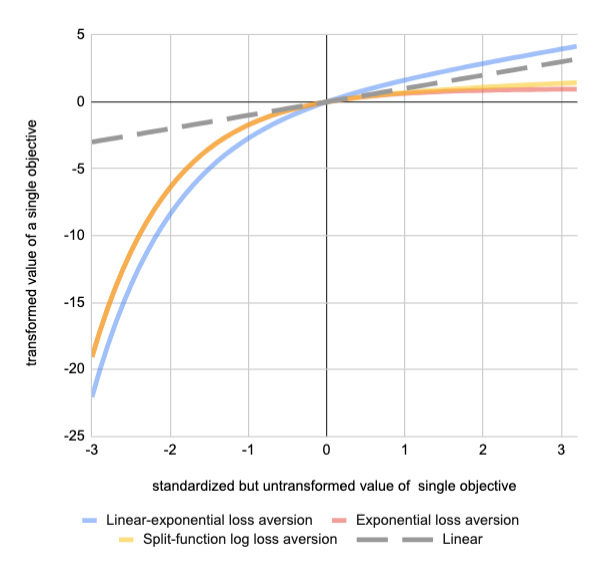
\includegraphics[width=\columnwidth]{output/transform_graph_2d.png}
  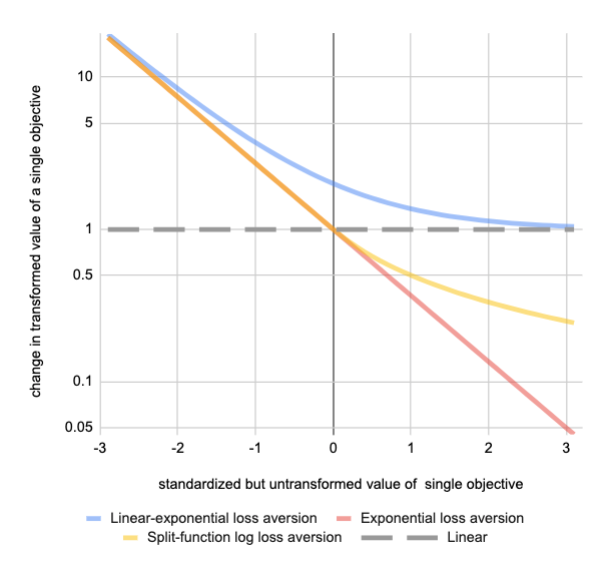
\includegraphics[width=\columnwidth]{output/transform_graph_2d_integral.png}
  \caption{Transform functions. Left: Each transform function is applied to the utility received from the environment for each objective. The output of each of these transform functions are summed together in a Maximize Expected Utility Model (Equation~\ref{eq:meu}). SEBA is not shown here because doesn't use an independent-objective transform function. Right: Change in $f(x)$ per unit $x$, with $y$ axis plotted on log scaling. Note that ELA and SFLLA produce greater-than-linear change in $f(x)$ in when $x<0$ and less-than-linear change when $x>0$. In contrast, LELA change never falls below 1.}
  \label{fig:transform_functions}
  \Description{Transform functions.}
\end{figure*}
%SFMLA might be the function that most intuitively expresses loss aversion, the idea that losses loom larger than gains:

%\begin{align}
%U^P(s, a)'= & cU^P(s, a) & \mathrm{ where \: U^P(s, a)>0} \\ \nonumber
%  &  2c U^P(s, a) &  \mathrm{otherwise} \\ \nonumber
%\end{align}

%(or we can write the following; which is better?)

%\begin{align}
%f(x)= & cx & \mathrm{ where \: x>0} \\ \nonumber
%  & 2c x &  \mathrm{otherwise} \\ \nonumber
%\end{align}

In SFLLA, there is a split in the function at $x=0$. It expresses a loss-averse function where losses will be stronger than gains:

\begin{align}
f(x)= & \ln(cx+1) & \mathrm{ where \: x>0} \\ \nonumber
  &  -\exp(-cx)+1 &  \mathrm{otherwise} \\ \nonumber
\end{align}

Additionally, by implementing a log rather than a negative exponential in the positive domain, the function retains relatively more weight on positive objectives.

The ELA greatly simplifies this approach, avoiding any split function at the cost of giving very little weight to any increase in values over 1:

\begin{align}
f(x)= &  -\exp(-cx)+1 \\ \nonumber
\end{align}

With LELA we add an $x$ term so that value continues to increase at least linearly at any point along the scale:


\begin{align}
f(x)= &  -\exp(-cx)+cx+1 \\ \nonumber
\end{align}

This still yields loss aversion at points less than zero but always provides that an increase in $x$ increases at least linearly in $f(x)$.


Finally, SEBA works using a different set of princples. Instead of branching depending on the value of $x$ the function treats the dimensions differently depending on their type: Depending on whether a dimension is part of the performance objective or part of the alignment objective.

For performance objectives the SEBA formula is linear:
\begin{align}
f(x)= &  cx \\ \nonumber
\end{align}
There is no differentiation between negative and positive areas of the measures of the performance objectives. This avoids the need for establishing a zero-point. Proper scaling is still needed.

For alignment objectives the SEBA formula is a square power function in order to express loss aversion. It is assumed that the values in the alignment objective can only be negative or zero.
\begin{align}
f(x)= &  -(cx)^2 \\ \nonumber
  &  \mathrm{ where \: x \leq 0}
\end{align}
The alignment related measures still have a “natural” zero-point, since they by definition are bounded at zero where no constraint violations are occurring. Therefore in case of safety related features it is not so difficult to establish where the zero-point is located at. Such measures would usually measure the deviation of something from a desired target value. Such measures have two main types:
\begin{itemize}
    \item The desired target value is zero (for example, zero harm, etc).
    \item Alternatively it might be a homeostatic setpoint (for example, optimal temperature, etc), so the measure is representing the negated absolute value of the deviation regardless of the direction of the deviation.
\end{itemize}

\subsection{Weight changes}

\subsection{Environment}

In every environment, agents a two objectives: a `primary' objective and an `impact' objective. We started with four environments reported in \cite{vamplew_potential-based_2021}. We wanted to understand how different aggregation functions could respond to perturbations in goal magnitudes. To do this, we repeated each experiment 9 times. The first time was with the original settings as in \cite{vamplew_potential-based_2021}. Then, we repeated this with each environment's primary utility feedback scaled by $10^{-2}$, $10^{-1}$, $10^1$, and $10^2$. The same range of scaling was then applied to the impact utility feedback.

\subsection{Benchmark}



Each of the proposed functions was compared against the best performing function in \cite{vamplew_potential-based_2021}, the `TLO$^A$` function, on the `R$^*$` metric from the same paper. The `R$^*$` arbitrarily scores a weighted combination of Primary and Impact objectives where one unit of Impact objective (always on a negative scale) is worth 50 units of the Primary objective.


